\section{Problem}\label{problem}

As the infrastructure of cloud computing grows rapidly, storage service providers use Key-Value Stores (KVS) 
in data centers to persist user data, with high throughput and low end-to-end communication latency~\cite{}.
Many users store their sensitive data (e.g., password, medical record) in these systems, while the protection 
of these data is not enough. 
Specifically, there are three dominant security properties in KVS: confidentiality, integrity and freshness.
(a) \textbf{Confidentiality} is to ensure that other unauthorized parties (e.g., malicious OS) cannot read the plaintext 
data of personal record in KVS. (b) \textbf{Integrity} is the property that the typical \textit{read} and \textit{write} 
operations of KVS cannot be tampered with, such as the changes to records in persistent storage. (c) \textbf{Freshness}
is the ability to detect stale state of data, in case a malicious KVS returns an older version of a request record.

Intel Software Guard eXtension (SGX), a popular security hardware on commodity available Intel CPUs, is promising 
to provide the first two security properties in KVS~\cite{}. SGX provides an abstraction of secure enclaves, which is a secured 
memory zone isolated from untrusted memories. By sealing enclave objects with secret SGX keys to untrusted memory (i.e., 
persistent storage on host) and unsealing encrypted objects to enclave, SGX ensures that in-enclave data is unavailable 
from the outside, even with a malicious OS or hypervisor~\cite{}.

Unfortunately, the freshness cannot be guaranteed by simply running KVS on SGX-enabled hosts. 
The problem lies in the lack of version check when an enclave loads objects from untrusted memory.
Figure \ref{fig:rollback} shows a typical rollback attack in a local scenario. The enclave calls the \textit{write} 
operation of KVS twice to store two different key-value pairs, respectively. When the enclave
requests for the latest value by calling \textit{read}, the attacker returns a previous version of value 
to the enclave. Since the enclave can only verify source of the returned object from the correct platform
through local attestation, the incorrect returned object cannot be detected by KVS users.

\begin{figure}
    \centering
        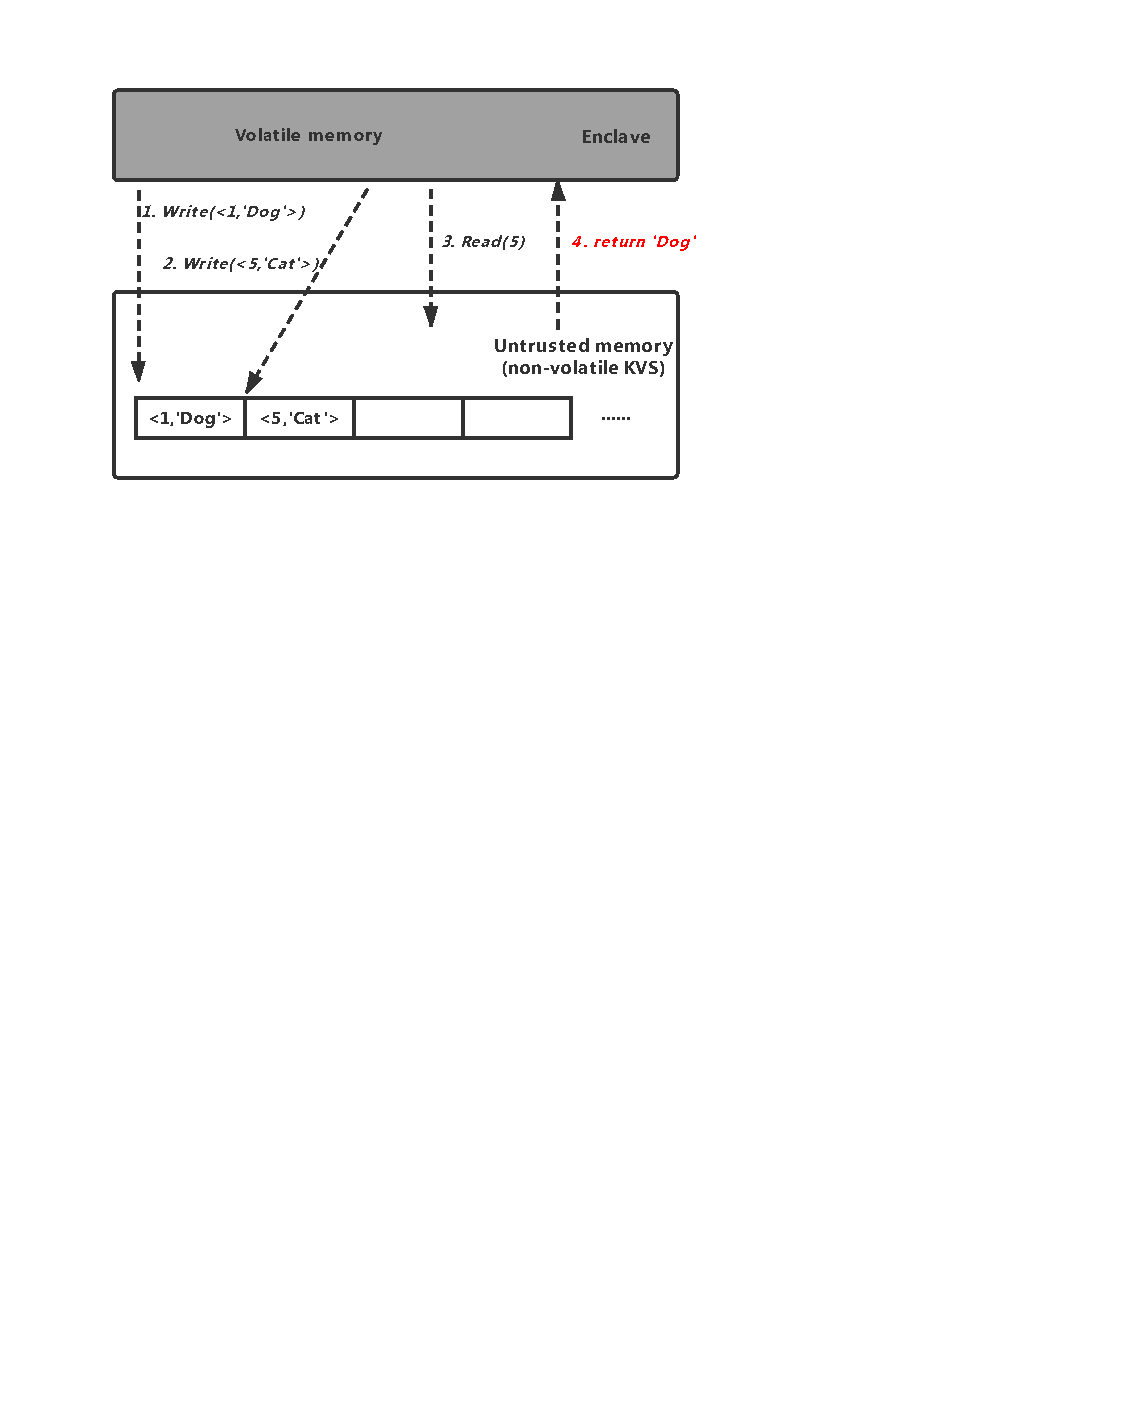
\includegraphics[width=.45\textwidth]{rollback.pdf}
        \caption[title]{An example of rollback attack towards KVS on SGX-enabled host. 
        The malicious OS returns an older version of value in KVS and the trusted enclave (in gray)
        cannot detect it. The records should be sealed/unsealed but we omit these operations for simplicity.}
        % \caption[title]{DAENet's scalability with increasing number of nodes.}
        \label{fig:rollback}
\end{figure}

To formalize, in addition to leverage the protection of SGX, we should also develop a freshness protection 
mechanism to protect against rollback attacks that replay old state of objects. In other word, we aim to expand 
the security protection of SGX from trusted volatile memory of enclaves to untrusted non-volatile memory of 
the outside, even when the system reboot, crash or during migration.
